\section{Implementation}

Having broadly introduced the framework within which our multi-agent simulation of the Kyoto Protocol operates, we can now elaborate on the specific implementation of individual components of our system. Implementation, in this sense, does not refer to Java constructs or actual code, but rather the design decisions that team members made during the project's development.

\subsection{Agents}

Agents are the intelligent actors within an environment that represent countries interacting with the Kyoto Protocol. The initial structure of our project groups allocated the distinct country behaviours discussed earlier in the report to groups of four people. Though this group structure became less rigid as the project progressed, each type of agent as originally outlined still approaches the Kyoto Protocol with markedly different strategies.

\subsubsection{Participants}

\paragraph{Annex I (Sustain)}

Agents implementing this type of strategy are meant to represent countries which are part of Kyoto and belong to Annex I group, but their emission targets are equal or higher than their emissions for the first Kyoto session.

The usual reason for this is that normally, while the first session started in 1990, the data used for setting the targets comes from 1990. During this period of history, many Eastern Bloc countries moved from heavily carbon-based economies to more environmentally conscious economies. Hence, even though Kyoto takes their former high carbon emissions into account, they have reduced their carbon output quite significantly since then, reaching or even exceeding the targets before the first session started. That, in turn, means that they do not have to reduce their emissions further during the first session.

\subparagraph{Strategy}

In order to make strategies distinct between Annex I sustain and annex I reduce, Annex I sustain countries will only remain a part of the Kyoto Protocol as long as they meet their targets. In the event that emission targets are lower than the acceptable output level for that participant, the country will attempt to reduce their emissions by investing in carbon reduction or absorption. Where funds, area or carbon output to reduce are unavailable, participants will leave the Protocol and become a `rogue state'. A small subset of participants are able to cheat (When their emissions exceed their targets, they report false values). If these cheating participants are caught multiple times, they may leave the Kyoto Protocol.


However, it is important to recognise that Annex I sustain countries did ratify the Kyoto Protocol when it was originally proposed and finalised. These countries' governments have expressed a desire to minimise their impact on the environment to some extent. It is with this in mind, that annex I sustain countries make sure that their overall emissions never rise above their starting levels. Any investment in industry to promote economic growth is offset by corresponding investments in cleaning industry or constructing carbon sinks.

On the other hand, Annex I sustain countries are reluctant to reduce their carbon emissions if it adversely affects their economic growth. Any reductions in emissions are because the country has judged that investment will be profitable when the resulting offset is sold on the carbon commodity market. This may seem like a bleak attitude for a set of countries to adopt, painting them as opportunistic and self-interested. However, this diversified the strategies our countries employ over the course of an entire varied simulation and more properly models Common Pool Resources, where individual interests are weighed against that of the collective.

The strategy contains three steps, taken every year in order:

\begin{description}
\item[1. Invest in industry] \hfill \\
Part of a year's budget is reserved for increasing the economy. Since this group represents mostly newly-developed countries, this is prioritised to promote long term growth.

As outlined earlier, the investment must be accompanied with carbon reduction or absorption, so that overall carbon emissions do not increase. To achieve that, a specific point is found for which total price of investments in industry and matching emission decrease is equal to the reserved budget.

\item[2. Sell carbon credits] \hfill \\
If the emissions of the country are lower than the target for a given year, the country will accumulate carbon offset, representing the `unused' emissions. The agents will attempt to sell all of these credits. Since carbon trading is essentially an open market, setting an average price can be challenging. To maximise profits from sales, the agents will start with a high asking price, reducing it gradually as the year progresses if no one is interested in buying, and increasing it when the sales go well.

\item[3. Invest in emissions reduction] \hfill \\
When a country has no credits to sell anymore, but there is still demand for carbon offset on the market, it may decide to invest in carbon reduction or absorption to generate additional carbon offset. First, it estimates how many of the generated units can possibly be sold during the current session, assuming the market price persists. If the estimated profit is higher than cost of the investment, the country will proceed with it. Should this occur, the country will reduce its emissions by the end of the session (reducing global output as an incidental benefit), and hence will end up with a target higher than actual emissions in the next session, just as in the previous one. If this is the case, it will stay in Kyoto for the next session.
\end{description}

\paragraph{Annex I (Reduce)}

In our project, we define Annex I reduce countries as participants whose current emissions are higher than their 1990 base targets, requiring them to prioritise the reduction of their carbon emissions. Good examples of such countries are the fifteen European countries.

For their behaviour, it was decided that the best approach was to design a mini simulation that would, once per simulation year, perform exhaustive testing on every possible country action, extrapolating emissions and industry growth for a number of years into the future. It then decides which sequence of actions results in the best outcome, with regard to maximizing economic growth while still meeting Kyoto Protocol targets, and then performs the action in the mini simulation that corresponds to the current year in the full simulation.

While simple in theory, in practice there is a very major hurdle; there are an enormous number of possible actions a given Annex I reduce country can take, all of which operate on a continuous scale. Every action has an almost infinite number of options that can be taken. For example, a country could choose to reduce their carbon emissions through absorption by spending 1\% of their available cash, or by spending 100\% of their available cash, or any number in between. They could then decide to buy vast amounts of carbon offset from the market, at any price, or put up sell offers. All of these actions can be performed in a single tick.

\subparagraph{Strategy}

In order to simulate the behaviour as efficiently as possible, some heuristics had to be implemented that would decrease the number of actions that could be taken to a manageable number. The first technique used was to take the previously continuous scale of actions and cut it into a variable number of discrete chunks. The number of chunks is variable upon how many years into the mini simulation have been calculated; the later into the simulation, the fewer chunks. This decreases the total number of branches produced while keeping as much accuracy as possible at the beginning of the simulation.

The next was to split the previously potentially infinite sequence of actions into a finite number of actions. To do this, it was decided to split each turn into three phases: the `reduce' phase, the `maintain' phase and the `sell' phase.

The reduce phase happens first. It checks whether our current carbon output is below our carbon target. If we are at or below our target, then nothing is done. However, if we are above our current target, the testing will branch off into combinations of three distinct actions. The carbon target will be met by either buying carbon offset from the market, by reducing the carbon output through investing in absorption and reduction or, if in particularly dire financial situation, by reducing the economic output of the country. Every time a branch occurs, a new `state' is created.

Before the maintain phase occurs, we compare every branched state with one another and check whether one state is objectively superior for every possible pair of states. For example, let a state have two attributes `Money' and `Carbon', where a higher `Money' and a lower `Carbon' is better. If state 1 has a `Money' value of 100 and a `Carbon' value of 50, and state 2 has a `Money' value of 90 and a `Carbon' value of 60, then state 1 is objectively better than state 2. Therefore we can immediately eliminate state 2 as a possible action. Alternatively, if a state 3 has a `Money' value of 110 and a `Carbon' value of 60, we cannot objectively say that it is any better than state 1 and thus cannot remove this from the simulation. By performing this culling, we can prevent our search space from getting too large and avoid going down paths where we can already tell there will be better alternatives.

Next is the maintain phase. As we are now guaranteed to be at least at or below our carbon target, the country can focus on improving its industry, which will eventually result in an increase in the available cash to spend. The simulation will branch off from each unculled state created in the reduce phase by first investing in industry (i.e. increasing our energy output, which in turn increases our \textsc{gdp}) by some amount and then by offsetting the extra carbon created by investing in absorption and reduction, or by buying the offset from the market. Once again, a cull is performed after all branches have been taken.

Finally there is the sell stage. Here, we reduce our carbon output (by investing in carbon absorption and reduction, or by shutting down factories) by a certain amount and then sell our newly created carbon offset at the highest possible price. Once again, all unrealistic states are culled.

The combination of these three phases makes up a list of possible actions for one year of the game. However, since a session lasts a number of years (at which point any accumulated carbon offsets are abandoned when new emissions targets are calculated), simulating the possible behaviour for a single year simply does not provide us with enough information to choose an ideal action path. The simulation needs to continue the internal projections up until either the end of the current session or until we reach a maximum number of branches.

Once this is over and we have a large number of end states, we can analyse our them to find the ones which can be objectively considered the best. This will be the one with the best economy and the lowest carbon output. When identified, we simply traverse our path back to the initial state and perform the action for the current year in the actual game.

As the Annex I reduce countries were deemed to be paragons of justice, some actions such as cheating and ignoring carbon targets weren't coded in. Overall, though, this method takes as much advantage as it can of the possible options available to a country, including utilising the market as much as possible. Unfortunately, due to computational constraints and the aggressive heuristics that were used, the absolute best possible action a country can perform in a given year doesn't tend to be taken although something very close will be performed.

This behaviour approach is an example of an uniformed breadth first general graph search where the ideal end state has no constraint other than to be superior to any other possible end state. This method means that the underlying algorithms can change in any way (e.g. the calculation of GDP) with only minimal changes to the behaviour code, while still being able to maximise economic growth and manage carbon output correctly.

\paragraph{Non-Annex}

The Non-Annex group is mainly composed of developing countries whose primary aim is economic growth. Since \textsc{gdp} growth is directly proportional to energy output in this project, the aim of Non-Annex countries is to increase its industry as much as possible. 

Investing in industry, and therefore growing a country's economy increases its carbon output at the same time. However, the Kyoto Protocol dictates that sanctions are not enforced on Non-Annex countries since they are not set targets to fulfill. They are therefore free to emit as much \CO as their industry requires.

Nevertheless, the Non-Annex behaviour was implemented such that they do care about the environment as well as their growth when cash is available in abundance.

The following keywords will be used to describe the general behaviour of Non-Annex countries:

\begin{description}
	\item[1. energy\_aim:] the energy output the country wants to reach by the end of the year.
	\item[2. times\_aim\_met:] how many consecutive times the energy output aim was met.
	\item[3. aim\_success:] variable that represents whether the country met its energy target or not.
	\item[4. green\_care:] variable that controls if the country cares or not about the environment.
	\item[5. green\_lands:] variable that controls whether the country has actually met its environmental commitments.
	\item[6. environment\_friendly\_target:] if it exists, variable that stores the country's carbon emission target. 
\end{description}

The country starts by having a policy of increasing its energy output, whilst trying to meet an internally set carbon emission target.

Each year, the country calculates the difference between its achieved energy output and the target aim that was set the previous year. The difference is then used to estimate the amount of money to invest in carbon industry each tick in order to reach the required energy output. Before the country proceeds with the investment, certain conditions have to be met:

\begin{itemize}
	\item It has the available cash to spend.
	\item If the country has decided to care about the environment, the increase in carbon output due to the investment should not lead to its emission exceeding the set target.
\end{itemize}

If the latter condition is not met, then the country tries to invest in carbon absorption or carbon reduction in order to decrease its carbon emissions. However, the country will switch to non environmental friendly policies if it does not have enough money.
 
Non-Annex countries take part in Clean Development Mechanisms. This allows Annex I and Non Participant countries to invest in Non-Annex countries in exchange for carbon offset.

In other words, Annex I countries use Non-Annex land area and carbon output to reduce their own emissions in order to meet their targets in the Kyoto Protocol. There are two ways in which countries can invest:
 
\begin{description}
	\item[Carbon Absorption] Decrease available land area, increase carbon absorption
	\item[Carbon Reduction] Carbon output decreases
\end{description}
 
The amount of carbon output to be changed/given to the Annex I country depends on whether the Non-Annex countries meets its energy output aim.

Carbon absorption offers are all accepted if the country is in an environmentally friendly phase (unless the available land area is at a minimum). 

\subsubsection{Non-Participants}

For the purposes of our simulation the rogue states are comprised of the \textsc{us}, who operate independently of one another, yet necessarily share certain actions and behaviours. 

\subparagraph{United States}

The United States agent uses a metric of ``greenhouse gas intensity'', defined as the ratio of emissions to economic output, measured in units of tonnes of \CO per million dollars of \textsc{gdp} to monitor its emissions. For example, using the 1990 data values, the intensity evaluates to 4,879,376/5,722,300 = 0.853 (3dp). To put in historical perspective, the Bush administration committed to reduce the intensity of greenhouse gas emissions by 18\% over the period 2002-2012.

In the real world it is the governing political party that makes any decisions regarding climate change mitigation, whose actions are in theory in response to the prevailing attitudes of the electorate, and so it is the case for the agent in our simulation. Every four years an election is held, with the initial party in power chosen at random. For simplicity's sake only the two major parties of the republicans and the democrats are represented. Broadly speaking, the democrats seek to increase the intensity value being targeted (which will have a greater impact on carbon reduction), whilst the republicans will target higher growth rates. The ultimate goal of the governing party is to gain re-election, which, as will be detailed below, is determined by the reductions implemented and economic growth over the period. The degree to which each of these effects the re-election chances of the incumbent party varies according to the prevailing attitude of the electorate, and the party in question. The republicans are more strongly punished and rewarded for economic growth, whereas the democrats are more strongly influenced by their carbon reduction efforts (reflecting the concerns of their core supporters). 

The agent has three overarching behaviour patterns controlling its attitude toward carbon reduction, represented by a integer variable between 1 and 10, where 10 is highly positive, and 1 is ambivalent. The real world representation of this being the prevailing attitude of the electorate, to which, in theory, the governing party responds and chooses actions in accordance with. This attitude variable is specifiable at the beginning of the simulation, and can change year by year. A more positive attitude results in more ambitious targets for the desired intensity level improvement chosen for the election cycle. Additionally, the more positive the attitude, the more influenced by success or failure in reaching or exceeding reduction targets the populace are, and the less they are influenced by lower economic growth. The opposite is true for more ambivalent attitudes.

The agent, as in reality, is not a member of the Kyoto Protocol at the start of the simulation, and thus is not subject to either monitoring or sanctioning. Despite its non-member status however, it is not entirely ambivalent toward carbon reduction. The agent has been designed so that through the natural oscillation of the party in power intensity levels will steadily decrease, and ultimately result in a decrease in absolute levels, which will result in the agent eventually joining the Kyoto protocol. Each year the agent checks to see if, were it part of Kyoto, would it have met its emission target. If for three years in a row the target is met then the agent joins Kyoto, conversely, if targets are not met for three years in a row after joining Kyoto, the agent will once again leave.

The winner of an election is decided by a function of the economic performance over the election cycle and the election year (the justification for the latter being the relatively short term memory of the typical voter), the carbon reduction measures undertaken, and the attitudes of the electorate and the party's core supporters toward these. After these factors have been taken into account, some level of randomness is introduced (perhaps one party has a particularly compelling candidate).

As the political party's re-election chances are determined by the levels of carbon reduction and economic growth achieved during the election cycle, it chooses targets for these (in the case of economic growth, assuming stable market conditions) in order to maximise this chance. The targets are initially based on the long term percentages reductions/growth rates achieved before being adjusted up or down. In order for an absolute decrease in emissions it is necessary for the emissions intensity to improve faster than economic growth. So, for an absolute decrease the targeted improvement in intensity must be higher than this. The desired improvement in the intensity level is thus taken at base to be the long term economic growth rate over the four year election period plus a value determined by the overall attitude of the electorate. E.g. If the year on year growth rate was 5\%, this would result in a 21.5\% compounded rate from the start to the end of the period. Targets are valid and acted upon over the four year election period in order to allow behaviors to adapt to the prevailing global economic conditions, in times where growth is strong, giving rise to more available cash, more investments toward carbon reduction are made, contrarily, during periods of poor economic growth more investments into the economy are made. 

Once the target is set, the agent sets about choosing actions. The agent aims to implement any actions over three years within the four year election cycle, allowing no action to be taken in one of the years if conditions are not favourable. If conditions are amenable, all available cash will be used. At the beginning of the election cycle the absolute carbon reduction required over the four year period (taking into account the expected \textsc{gdp} growth) is calculated. The goal in absolute terms for each of the three years is then set. The agent will attempt to fulfil its commitments during the first 99 ticks of the year (assuming a year is 100) through the clean development mechanism (\textsc{cdm}), or subsequent to Kyoto membership, through trading carbon offset with other agents. Before implementing any action, the agent evaluates whether the benefit to their election chances will be increased more by taking the action in question or an alternative. On the last tick of the year, if the targets for carbon reduction or \textsc{gdp} growth have not been met, then the agent will take appropriate action through the carbon reduction and absorption mechanisms, or through investing in industry. The party will take measures to meet either its reduction or growth targets first depending on, once again, the projected effect the meeting/not meeting one will have on their reelection chances. Then use any remaining cash available to meet (if possible) the remaining target. If both targets have been met, they will spend the remainder on their preferred action.

\subsection{Participant Actions}

\subsubsection{Carbon Reduction Handler}

The cost of carbon reduction for a country depends on its ratio of carbon output to energy output, which can be described as a dirty industry percentage:

\begin{align*}
\mtext{Dirty Industry} = \mtext{Carbon Output}~/~\mtext{Energy Output}
\end{align*}

The less dirty our industry is, the more expensive it gets to clean it further. Therefore, it is reasonable to use a measure of clean industry:

\begin{align*}
\mtext{Clean Industry} = 1 - (\mtext{Carbon Output}~/~\mtext{Energy Output})
\end{align*}
 
The relationship between the cost of reducing carbon output by one unit and the percentage of 
clean industry at a given moment is given in Figure~\ref{fig:carbon_reduction}:

\begin{figure}[h!]
	\centering
	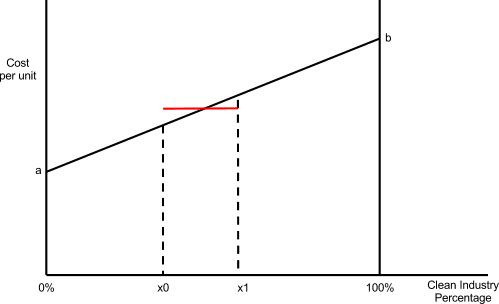
\includegraphics[width=0.6\textwidth]{img/carbon-reduction.png}
	\caption{Price of carbon reduction}
	\label{fig:carbon_reduction}
\end{figure}

Where:
\begin{itemize}
	\item a: cost of reducing carbon output by 1 with 0\% clean industry (min cost, constant)
	\item b: cost of reducing carbon output by 1 with 100\% clean industry (max cost, constant)
	\item x0: clean industry percentage before investment
	\item x1: clean industry percentage after investment
\end{itemize}

 
Hence, we can calculate cost of single unit investment at specific clean industry percentage using the following formula:

\begin{align*}
\mtext{Unit Cost} = a + ((b - a) * x)
\end{align*}

Since the cost will increase linearly with every unit invested, we can find the average cost for the whole investment as the average of the initial and final cost (based on the x0 and x1 values). This is represented by the red line on Figure~\ref{fig:carbon_reduction}.
 
\begin{align*}
\mtext{Average Cost} &= ((a + ((b - a) * x1) - (a + ((b-a) * x0))) / 2 \\
&\Leftrightarrow \mtext{Average  Cost} = (a + ((b - a) * (x1 - x0))) / 2
\end{align*}

We can now calculate the total cost of a carbon reduction action by multiplying the average unit cost by the amount required by the country.

\paragraph{Reduction Cost Estimation}

This `inverse' operation is mathematically solved with a quadratic equation. However, this is difficult to implement and is error-prone due to double arithmetic in Java. Instead, a binary search bounded between 0 and the current carbon output was used. In each iteration, the function calls the \texttt{getInvestmentRequired()} function with a hypothetical carbon reduction as parameter. It then adjusts the amount of reduction the country will receive depending on whether the returned value is higher or lower than the actual investment. Since there are 30 iterations, it will produce a an accurate result providing the current carbon output is less than 2$^{30}$.
  
This function allows participants to estimate and compare the profitability of a carbon reduction investment. As it is not used by the investment function itself, the lack of absolute accuracy is not crucial.

\subsubsection{Carbon Absorption Handler}

The implementation of carbon absorption is very similar to that of carbon reduction investment. Here, the cost of forestation is inversely proportional to the percentage of area that is unoccupied with respect to entire land area of a country:

$$
Occupied~Area= 1 - Arable~Land~Area / Land~Area
$$

The cost of this action is calculated in the same way as for carbon reduction, with the only difference being the constant values for a and b. Additionally we also now need to calculate the area occupied by newly planted trees. This is done by using a constant specifying how much forest area is needed to absorb single unit of carbon, which is then multiplied by the amount of carbon absorption done.

\paragraph{Absorption Cost Estimation}

Again, the implementation is the same as in the case of carbon reduction. There is only one difference, which causes a slight problem. Binary search requires lower and upper bound, and, potentially, carbon absorption can be as high as possible (providing a country has sufficient land and funds). Hence, we needed to use some upper bound to allow using binary search algorithm.

Even though a country can invest in carbon absorption as much as it wants, it does not make much sense for it to exceed carbon output, and shouldn't be realistically possible providing reasonable constants for prices. Hence, the upper bound which is used here is a difference between carbon output and carbon absorption of a country, so that, for maximum investment, the function will return absorption change which forces actual emissions to atmosphere to 0.

Still, this will produce false results where investment is high enough to potentially increase carbon absorption beyond carbon output. Again, this is just an additional function for countries to make writing strategies easier and make them more interesting. Since there is no way around it, it was decided to allow this potential inaccuracy.

\subsubsection{Energy Handlers}

Each country in our simulation has the ability to influence its economy by investing or reducing its carbon industry. This functionality is provided to each participant through an instance of the energy handler. Unlike the carbon handlers, the price of a unit of investment in your carbon industry is a constant defined at the start of the simulation. In addition, there is no cap on the amount a country is allowed to develop its industry. 

The cost of an investment for a given desired growth can be modelled by the following linear function:

$$
Cost = Growth \times Price~of~Carbon~Investment
$$

Similarly, each participant can also use the handler to query how much economic growth can be achieved for a given cost:

$$
Growth = Cost / Price~of~Carbon~Investment
$$

Using these two functions, participants can make an informed decision on whether to invest in their industries or decide to reduce it. A country can increase its \textsc{gdp} by building factories which in turn will give them more money to spend in the following year. However, its carbon emissions will also increase as a result.

On the other hand, a country can decide to close down factories. This is a cost free method of reducing carbon emissions, though it also leads to a contraction of its economy and \textsc{gdp}. 

\subsubsection{Carbon Reporting}

Each country is required to submit yearly reports of their \textsc{ghg} emissions. The timing of reports is coordinated by the monitoring service to ensure synchronicity with the targetting service and consistency between separate agents. Each agent submits its report by acting on the environment, altering the shared state. They also update an internal record of their emissions reports, to make sure that agents can properly query their own history.

Countries are given an opportunity, at this juncture, to cheat and falsify their emissions reports by reporting incorrect carbon output data. If a country has exceeded its emissions target, correctly reporting their carbon emissions will guarantee that they receive a missed target sanction, which is a more severe target in the following year. Countries can attempt to avoid this sanction by reporting lower than their actual emissions. However, there is a chance that their emissions report will be monitored. If it is, they will be subjected to financial sanctions, arguably more damaging than severe emissions targets. This tradeoff must be evaluated by each country's behaviour.

\subsubsection{Joining \& Leaving Kyoto}

In our simulation platform, we allow countries to leave and join the Protocol. In order to replicate the Kyoto country categories, it was decided to offer participants three distinct levels of subscription to the simulation using Java enumerated states. Each of these give access to a different set of possible actions as described previously. Using this functionality, we can emulate real world scenarios such as Canada leaving the Protocol.

\subsection{Services}

\subsubsection{Trade Protocol}

The Trade Protocol allows participants to engage in trading of carbon offset or Clean Development Mechanism (\textsc{cdm}) investments in other participants/countries. The Trade Protocol class inherits from the \texttt{FSMProtocol} class provided in the Presage2 \textsc{api}, which is an implementation of agent protocols, used by agents to communicate with one another.
 
The trade protocol can be used for both carbon trading and Clean Development Mechanisms. The type of message that the trade protocol deals with is an object of type \texttt{OfferMessage}. The \texttt{OfferMessage} object has information of who initiated the conversation and who broadcast the offer in the first place and all the information about the quantity and unit cost of the offer. The quantity refers to the total, in tonnes of carbon offset, that are being offered. The unit cost refers to the price per ton. The total cost of the offer is the product of these two values.

When a participant broadcasts a carbon trading offer then the type of the Offer (also another 
object that \texttt{OfferMessage} encapsulates) is set to either:
 
\begin{itemize}
	\item \texttt{BUY}: If participant wants to buy carbon offset.
	\item \texttt{SELL}: If participant wants to sell carbon offset.
\end{itemize}

For Clean Development Mechanisms, the trade protocol allows the participant to advertise whether they want other countries to invest in their industry to reduce carbon emissions. When a participant wants to advertise about \textsc{cdm} then the following types need to be assigned to the \texttt{OfferMessage} Offer type:

\begin{itemize}
	\item \texttt{INVEST}: participant wants to invest in another country.
	\item \texttt{RECEIVE}: participant is asking for other countries to invest in their industry/country.
\end{itemize}

It is also further specified whether the form of \textsc{cdm} is for carbon reduction or carbon absorption, which restricts the participant to choose the following investment types:

\begin{itemize}
	\item \texttt{ABSORB}: Whether the investment will be used to reduce carbon emissions by investing in absorption techniques.
	\item \texttt{REDUCE}: Whether the investment will be used to reducing carbon emissions via investing in carbon reduction techniques.
	\item \texttt{INVALID}: If investment type does not exists as it is a buy or sell carbon offer.
\end{itemize}

Trade Protocol works in the following ways:

\begin{enumerate}
	\item A participant who is willing to engage in a trade sends a broadcast message using the \texttt{network} object provided to every agent. This message contains information about the trade as they wish it be carried out.
	\item Another participant who is interested in the offer broadcasted can start a protocol conversation with the broadcaster. They can reply with slightly altered offers, to simulate a minor form of negotiation.
	\item The broadcaster can then accept or reject the offer that is proposed by the initiator.
\end{enumerate}

%
%	Can the english in this bit be checked
%

The process is illustrated in Figure~\ref{fig:protocol}: ~\subref{subfig:protocol1} shows agent Peter mulicasting a sell offer to all agents; in \subref{subfig:protocol2}, agents Tom and Yiannis are interested in the offer, and so initiate the \texttt{TradeProtocol} with peter; finally, in \subref{subfig:protocol3}, agent peter decides to accept the offer initiated by Yiannis.

\begin{figure}[h!]
        \begin{subfigure}[b]{0.3\textwidth}
                \centering
                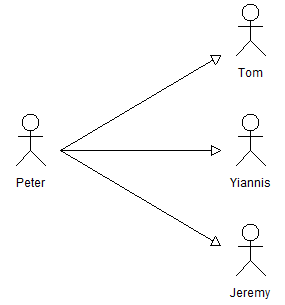
\includegraphics[width=\textwidth]{img/protocol1.png}
				\caption{}
				\label{subfig:protocol1}
        \end{subfigure}%
        ~ %add desired spacing between images, e. g. ~, \quad, \qquad etc. 
          %(or a blank line to force the subfigure onto a new line)
        \begin{subfigure}[b]{0.3\textwidth}
                \centering
                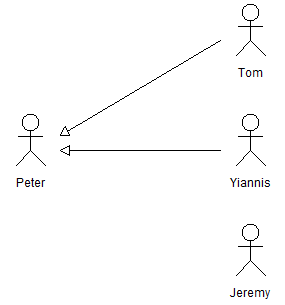
\includegraphics[width=\textwidth]{img/protocol2.png}
				\caption{}
				\label{subfig:protocol2}
        \end{subfigure}
        ~ %add desired spacing between images, e. g. ~, \quad, \qquad etc. 
          %(or a blank line to force the subfigure onto a new line)
        \begin{subfigure}[b]{0.3\textwidth}
                \centering
                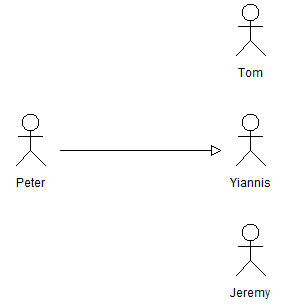
\includegraphics[width=\textwidth]{img/protocol3.png}
				\caption{}
				\label{subfig:protocol3}
        \end{subfigure}
        \caption{\texttt{TradeProtocol} action diagram}\label{fig:protocol}
\end{figure}

In the event that a trade is unable to be carried through to the end, possibly caused by one of the countries not having enough available funds to complete the transaction, the trade can be reverted, and the involved parties are refunded.

\paragraph{Trade Protocol State Machine}

The protocol has two different state machines that are used by the initiator and the broadcaster. The state machines are as follows: 

%
% FIX THE POSITION OF THESE FIGURES
% cs2309: What is wrong with them?
%

\begin{figure}[h!]
	\centering
	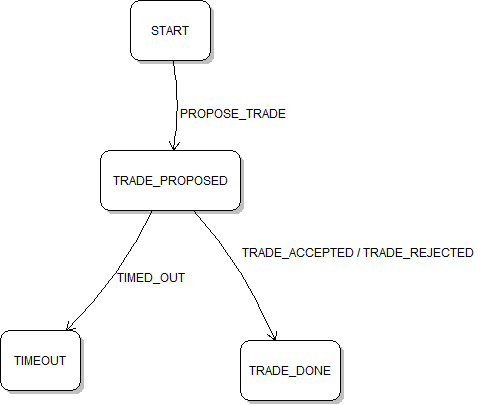
\includegraphics[width=0.6\textwidth]{img/protocol-fsm-1.png}
	\caption{Initiator \textsc{fsm}}
	\label{fig:protocol-fsm-1}
\end{figure}

\begin{figure}[h!]
	\centering
	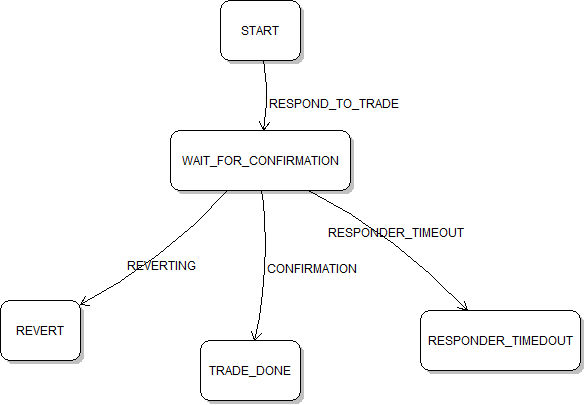
\includegraphics[width=0.6\textwidth]{img/protocol-fsm-2.png}
	\caption{Responder \textsc{fsm}}
	\label{fig:protocol-fsm-2}
\end{figure}

Figure~\ref{fig:protocol-fsm-1} and ~\ref{fig:protocol-fsm-2} shows the state machines used by the Initiator and Responder respectively along with the transitions labelled on the arrows. The transitions in an \texttt{FSMProtocol} happen when a participant receives a message.

\paragraph{Initiator FSM}

Both the initiator and the responder have a single \texttt{START} state as required by the \texttt{FSMProtocol}. The initiator has two end states, which are \texttt{TIMEOUT} and \texttt{TRADE\_DONE}. Each transition results in the participant performing a particular action of sending back a message to the responder, which makes the responder transit to the next state.

\begin{description}
	\item[1. \texttt{PROPOSE\_TRADE}:]
	When the participant responds to the offer, it transitions to the \texttt{TRADE\_PROPOSED} state and sends a Unicast message to the broadcaster waiting for its response.
	\item[2. \texttt{TIMED\_OUT}:]
	From the \texttt{TRADE\_PROPOSED} state a timeout of 3 ticks is set so that the initiator times out into an error state.
	\item[3. \texttt{TRADE\_ACCEPTED}:]
	If the responder accepts the trade proposal, the Trade Protocol handles the trade completion through a function called \texttt{handleTradeCompletion()}. If anything goes wrong while handling the trade completion then the participant (initiator) transits to the \texttt{TRADE\_DONE} state by sending a Unicast message to the responder to revert the changes. If the handling of trade completion works well then the participant transitions to the end state \texttt{TRADE\_DONE} by sending a confirmation message to the responder.
	\item[4. \texttt{TRADE\_REJECTED}:]
	If the trade was rejected by the responder then the participant (initiator) transits to the \texttt{TRADE\_DONE} state by sending a confirmation unicast message to the responder that it has received the message.
\end{description}

\paragraph{Responder FSM}

Figure\ref{fig:protocol-fsm-2} shows the \textsc{fsm} that is used by the responder. Upon receiving a message form the initiator. There is only one \texttt{START} state and the three end states are \texttt{REVERT}, \texttt{TRADE\_DONE} and \texttt{RESPONDER\_TIMEOUT}. Similar to the initiator, the transitions happen with the participant sending a unicast message to the initiator agent.
 
\begin{description}
	\item[1. \texttt{RESPOND\_TO\_TRADE}:]
	This transition occurs when the initiator spawns a message, which makes the responder transition to the \texttt{WAIT\_FOR\_CONFIRMATION} state. If the responder accepts the exchange then it transitions to the next state by sending a unicast message to the initiator that it accepted the trade, otherwise it transitions to the next state by sending a unicast message to the initiator that it has rejected the offer. Once the participant makes the decision to accept the offer then the \texttt{handleTradeCompletion()} function is called to adjust the carbon offset and cash of the responder. If things fail for reasons such as not enough cash exception from the responder then the changes made to the responder’s carbon offset and available to spend will be reverted. Nevertheless, a reject message is sent to the initiator to inform him that the trade was unsuccessful.
	\item[2. \texttt{REVERTING}:]
	If the initiator fails in completing the trade for reasons such as not enough cash exceptions, then the initiator reverts itself and sends a message to the responder. Once the responder receives this message then it goes to the \texttt{REVERT} state via the \texttt{REVERTING} transition. There, it reverts all of the changes since the start of the conversation.
	\item[3. \texttt{CONFIRMATION}:]
	This is a transition to from \texttt{WAIT\_FOR\_CONFIRMATION} to the end state \texttt{TRADE\_DONE} state. This transition happens when either trade was successful or was unsuccessful (i.e. the responder rejected the trade in the first place).
	\item[4. \texttt{RESPONDER\_TIMEOUT}:]
	Timeout condition of 3 ticks from \texttt{WAIT\_FOR\_CONFIRMATION} state to the \texttt{RESPONDER\_TIMEDOUT} state, which is the end and error state of the responder.
\end{description}

\subsubsection{Time Service}

The time service is an environment service, extending Presage2's existing environment interaction classes and development framework. It allows for coordination of time-based events and synchronises various features within our Kyoto Protocol simulation. Although Presage2 does have existing objects (SimTime) which can be used to attain simulation time, this is an absolute value in discrete logical time since the beginning of the simulation. It therefore does not take into consideration the variety of chronological distinctions the Kyoto Protocol requires, such as subdivisions into years and sessions.

It was initially decided to use a global service. It would perform most of the logic integral to coordinating time-driven activities, and would be layered on top of Presage2's integrated SimTime object. However, it is necessary for agents to be able to query for information regarding the current year and session in order to make important strategic and behavioural decisions. Presage2 enforces that agents (participants) are unable to communicate directly with global services. While agents can act on the environment and affect services, performing the reverse is somewhat more complex.

At this stage, it would seem a participant time service would be more appropriate, since participant services can communicate directly with agents. However, another key functionality of the time service is the publishing of new events, both for the end of years and sessions, which trigger key monitoring, sanctioning, reporting, and architectural actions essential to the managed nature of the Kyoto Protocol. Unfortunately, implementation is not in place within Presage2 for participant services to generate (or interact with) the EventBus class, the object essential to publishing or receiving events.

With these restrictions in mind, the time service was subdivided into two separate services. The participant service communicates with agents and relays information regarding the current year and session, among other minor time-related information gathering tasks. The global service is the backbone of the time service, generating new year and session events for the monitoring and targeting services to hook onto. It also carries out calculations to derive the current year and session from the discrete simulation time and communicates this information to the participant service.

Both classes extend from Presage2's predefined EnvironmentService class, and use Google's Guice injection systems for initialisation and, in the global service's case, to register with the EventBus.

\subsubsection{Monitor}

The monitor's purpose is to regularly check whether countries are meeting their targets and randomly check for false carbon emission reports. If either case is true, a scaling sanction is applied to the country.

We were initially unsure whether the monitor should be an independent agent or an environment service. We settled on making it a service, so that it could listen to an event that would trigger the monitoring as agent are unable to do so.

When countries are initialised they subscribe to the monitor either as Annex I or Non-Annex. Although only Annex I countries are monitored, the Non-Annex countries list was required to fix an issue with events at the end of a year happening in the right order. Indeed, countries were calling for their targets for the next year to be updated before the monitor could compare the results for the previous year against its previous targets. This was fixed by updating targets after the monitoring function in the Monitor service.

Every year the monitor charges the Annex I countries a tax, which is used to perform the monitoring action on randomly selected countries. If the monitor runs out of money, it cannot monitor and countries are free to behave without fear of sanction (although this information is hidden).

\subsubsection{Carbon Target}

The carbon target service is responsible for reducing the world carbon emissions through the calculation of targets for all Annex I Kyoto members. Within the Presage2 simulation it is set up as a global service, this enables it to listen on an event bus and run independently from the country agents.
 
All target calculations are triggered by the end of year event generated by the time service via a method call from monitor.

How the worldwide targets are calculated:
\begin{align*}
\mtext{Reduction Coefficient}&= 0.95 ~ (5\%~reduction) \\
s &= \mtext{current session number}\\
\\
\mtext{World session target}[s] &= \mtext{world session target} [s - 1] \times \mtext{Reduction Coefficient}\\
\mtext{Kyoto target}[s] &= \mtext{world session target}[s] - \mtext{total non annex I output}[s - 1]\\
\end{align*}

Annex I target calculations, in each session:

\begin{align*}
y &= \mtext{current year number}\\
\\
\mtext{Country Proportion}[s] &= \mtext{country output}[y - 1]\\
&~~~~/~(\mtext{world output}[y - 1] - \mtext{non annex I output}[y - 1])\\
\mtext{Country Session Target}[s] &= \mtext{Kyoto target}[s] \times \mtext{country proportion}[s]\\
\end{align*}

In each Year:

\begin{align*}
\mtext{Session Progress}  &= \mtext{current year in session}~/~\mtext{number of years in session}\\
\mtext{Session Target Difference}&= \mtext{session target}[s - 1] - \mtext{session target}[s]\\
\mtext{Year Target}&= \mtext{session target}[s - 1] - \mtext{session target difference}\\
&~~~~\times \mtext{session progress} - \mtext{penalty}\\
\end{align*}

In the event that a session target is needed from before session 0, world data from 1990 is used in its place. This models the Kyoto Protocol's basis of its initial targets.
 
To avoid unfairness and promote economically feasible targets, as is negotiated in the real Kyoto Protocol, we restricted the maximum reduction across a single session to be 10\% of total emissions. Without this limitation, large emissions from rogue states can cause targets for Annex I targets to reduce unreasonably quickly. To handle unusual corner cases that may cause a country's session target to be higher than its previous session target (possibly due to drastic reductions by other member states, or large emissions from rogue states) we have restricted session targets so they cannot have a higher value than the previous session target.
 
Only Annex I countries are calculated a target. However, both Non-Annex countries and rogue states have an impact of target assignment. As can be seen in the above formulas and in keeping with the objects of the Kyoto Protocol in reality, the aim for a single session is to reduce global \CO emissions by 5\%. After calculating the desired output for this session, the targeting service calculates the required reduction from member states, assuming Non-Annex countries and rogue states continue producing the same amounts of \CO.

\paragraph{Implementation}

The carbon target service retains all the necessary data required for the above calculations in a private arraylist. Year targets are also set using a package protected method in the \texttt{AbstractCountry} superclass.
 
Within our simulation it is possible for countries to report false carbon emissions. Each year monitor service decides to monitor a subset of the countries. If a country is found to have reported a false value, its \texttt{UUID} is added to a list of cheaters. This list is then passed to \texttt{CarbonTarget} each year by \texttt{Monitor}, and is referenced when querying carbon output values for the target calculation.
 
Some countries (for example the \textsc{us}) may wish to join Kyoto at some point during the simulation. Since individual year targets are interpolated values dependent on session targets, and session targets are dependent on global emissions and each country's status as a rogue or member state, having a country join the Kyoto Protocol mid session is, in our simulation, extremely difficult. Each country's target would need to be recalculated and this introduces potential conflicts with existing strategies that the member state AIs have chosen. As a solution to this, we decided that rogue states could only join Kyoto at the beginning of a new session. Any rogue state that attempts to join the Kyoto Protocol in the middle of a session will be put on a waiting queue and will automatically be registered and become an Annex I country at the beginning of the next session.

We decided that any rogue state joining the Kyoto Protocol would automatically become an Annex I country for two reasons. One was the simplification of the rejoining process, which had already become extremely complex. Also, when compared to reality, it seemed reasonable that any country which left the Kyoto Protocol and then rejoined at a later date would then be assigned targets and monitored, to ensure that the system was not abused for financial gain. The US, the only major nation that did not ratify the Kyoto Protocol at its inception, would be an Annex I country regardless, were it to participate.

Leaving Kyoto is another potential action taken by member states, as seen in reality when Canada departed the Kyoto Protocol in 2011. When a member state leaves, its output is immediately recognised as that of a rogue state, and its departure has an effect on the setting of new session targets after the current session ends.   
 
Joining and leaving the Kyoto Protocol, as well as other actions such as reporting \CO emissions to the monitoring service, are implemented via action handlers, integrating with Presage2's defined structure for agents communicating with non-participant services and the multi-agent systems design paradigms regarding agent interaction with the environment.

\subsubsection{Market}

Our Kyoto simulation integrates a very basic emulation of the state of the financial markets. Each year, the market state will be determined randomly and affects by how much a country's \textsc{gdp} will change. By default, there is a 10\% probability that the economy is stable, 10\% that it is in recession and a 80\% probability that it is in a period of growth, but these can be changed by the user when running a new simulation.

\subsection{Game Balancing}

As we have seen, the game is made up of a series of mathematical functions, many of which rely on a set of constants (eg. \texttt{GROWTH\_SCALAR}, \texttt{MAX\_GDP\_GROWTH}). Varying and balancing these constants allows us to create varied and accurate simulations. These can be either initialised at compile time, or injected by the Kyoto \textsc{ui} at runtime, in order to run a wide range of different scenarios.

The balancing of these constants was not a simple task, since changing one may have an impact on others. The following 3 facts were used as a starting point for calculating suitable values for some of the constants:

\begin{enumerate}
\item Each country has an emission target of -5\% from their base year.
\item Countries typically invest 0.5\% of their \textsc{gdp} in developing clean industry every year.\cite[Figure 12]{PEW-Environment}
\item It takes ~0.0156 km$^{2}$ of trees per tonne of carbon absorbed.\cite[Accessed Jun 2012]{Trees-in-Trust}
\end{enumerate}
  
From 1, we can derive: 

\begin{enumerate}[resume]
\item The likely energy change per year (0.05\%)
\item \textsc{gdp} rate, since we can work out the energy difference
\end{enumerate}

From 2, we can derive:

\begin{enumerate}[resume]
\item The amount of cash each country gets each year
\item Sanction rate and tax rate as proportion of cash
\end{enumerate}

From 4 and 6, we can derive:

\begin{enumerate}[resume]
\item The cost of carbon reduction and absorption.
\end{enumerate}

\subsection{Kyoto UI}

The Kyoto \textsc{ui} is a web interface designed for instantiating and editing Presage 2 simulations. Web technologies used include an Apache web server, \textsc{php}, \textsc{html} and Javascript. Combined with a few additional libraries, these technologies provide the functionality required to display rich pages which allow for good visual representation and easy editing of data.

\subsubsection{Inception}

Initially, investigations into a \textsc{ui} began to solve the problem of a large amount of incoming data. This data can be used to initialise the agents and simulation in order to more effectively model the Kyoto Protocol in different global environments.

Each agent requires ten fields of initialisation data, and data was collected for 179 countries, so a Comma Separated Value (\textsc{csv}) file could be used to export data for analysis.

A \textsc{csv} file including simulation parameters is used alongside the country data, to initialise the simulation. This data sets up the document in mongodb that Presage2 is expecting.

It quickly became clear that the KyotoUI could be more than a database initialisation program and with some improvements it could become a dashboard for politicians and economists and have commercial value. The further development to KyotoUI is inspired by the idea that we are applying an accessible front to a specialised Presage2 simulator (Kyoto) in order to setup and report on simulations. Making simulations easier to initialise and interpret, means users can more efficiently analyse large numbers of simulations, and draw better conclusions on whether the Kyoto Protocol could work such as these will last in the long run.

Some additions made to the Presage2 simulation collection were to add a description and author field, to better represent the multi-user approach and have better record keeping. Also in the simulations collection is a list of all the starting data kyoto to load the necessary, under a branch named “countries”.

\subsubsection{Database Implementation}

The mongo database is interfaced using an Object Document Mapper (\textsc{odm}) library called mongorecord. This wraps interfaces for querying and writing the collections in the database with \textsc{php} classes which can be instantiated and used throughout the project.

\subsubsection{Simulation Initialisation Data Import and Export}

In order for any simulation to have a starting point, data files must be imported containing information such as how long the simulation should run for and the data is required to set up each of the agents. Presage2 has a command line interface which can be used to create simulations in the database and add parameters to them. The structure of these simulations in the database was used as a framework to import \textsc{csv} files of data to create simulations in the same format as generated by the Presage2 \textsc{cli}.

\subsubsection{CSV Import and Export Functionality}

To get data in and out of the system \textsc{csv} files are used. This is a convenient method of transferring data as the \textsc{csv} file can be opened and edited in spreadsheet software such as Microsoft Excel. Country data is inserted into the simulations, as are parameters from `default' \textsc{csv} files. Once these are in the database, the \textsc{ui} can copy and edit them. Simulations can then be exported as a backup or to transfer them to another database. This functionality underpins the whole simulation by providing an easy way to get a huge amount of data in and out of the system quickly, easily, and reliably.

\subsubsection{Simulation Editor UI}

Once data has been imported from the \textsc{csv} file it may be necessary to make new simulations by changing parameters etc. This is one of the main tasks of the web \textsc{ui}, to make this editing visually comprehensive and easier than manually editing the \textsc{csv} file or the database entry.

\subsubsection{Agent (Country) Data}

Agents in the simulation represent countries, and in order for the simulation to be as realistic as possible, these are modelled on real countries with parameters describing land mass etc. stored in the database. It is useful to edit some of these parameters, such as the percentage of land mass available for green development, to investigate what happens in a simulation given agents with different parameters. The \textsc{ui} features a page specifically for editing countries which displays a clickable map of the world with a dropdown menu for country selection. This way all countries within a single simulation can be edited dynamically.

\begin{figure}[h!]
	\centering
	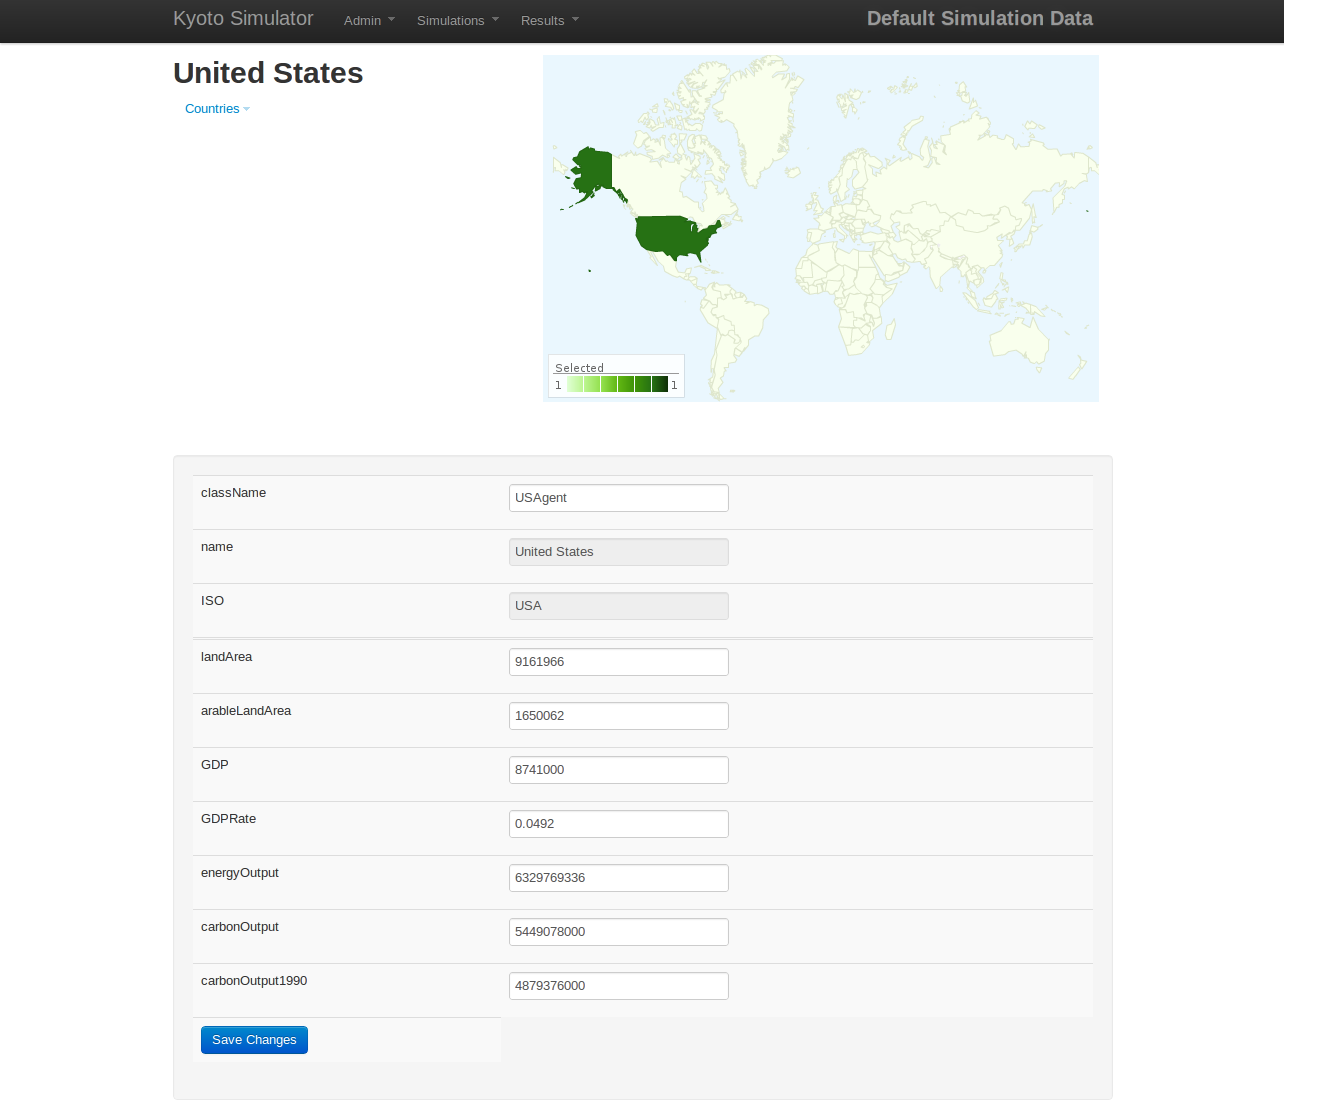
\includegraphics[width=0.9\textwidth]{img/ui1.png}
	\caption{}
\end{figure}

\subsubsection{Simulation Data}

Once imported, simulation data resides in a collection within the database. The \textsc{ui} provides a list of all simulations stored in the database with some basic information about the simulation displayed in the list. Next to each simulation is a menu which allows you to do several things with the simulation: view (detailed view of the simulation in the database),  export the simulation as a \textsc{csv} file, edit the simulation, copy it, or delete it.

\paragraph{Simulation Overview Page}

\begin{figure}[h!]
	\centering
	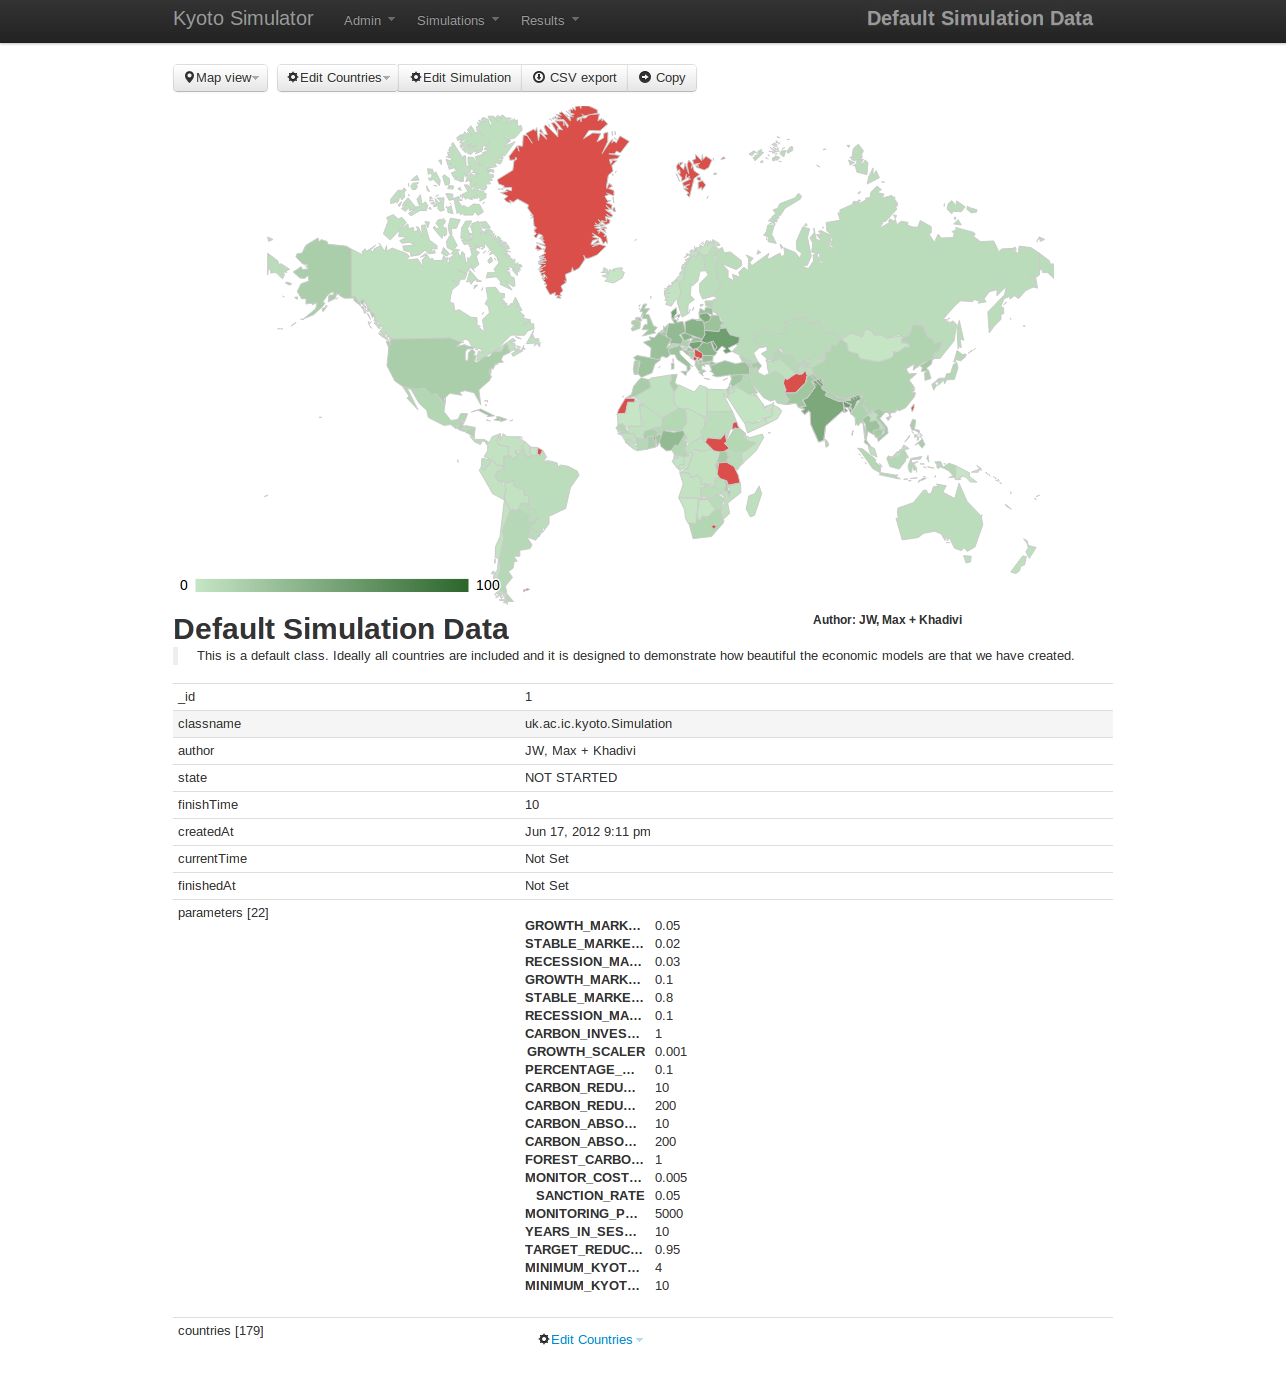
\includegraphics[width=0.9\textwidth]{img/ui2.png}
	\caption{}
\end{figure}

The simulation overview page displays a world map using colour to indicate the values of a selected parameter for each country (default is arable land area percentage). There is a drop down menu (Map View) which allows changing of the parameters displayed on the map. Below this is a table displaying a detailed output of all the simulation data from the database. This page also links to the \textsc{csv} export feature, copy feature, edit simulation page and a dropdown is present to allow editing of all the countries within the simulation.

\paragraph{Simulation Edit Page}

\begin{figure}[h!]
	\centering
	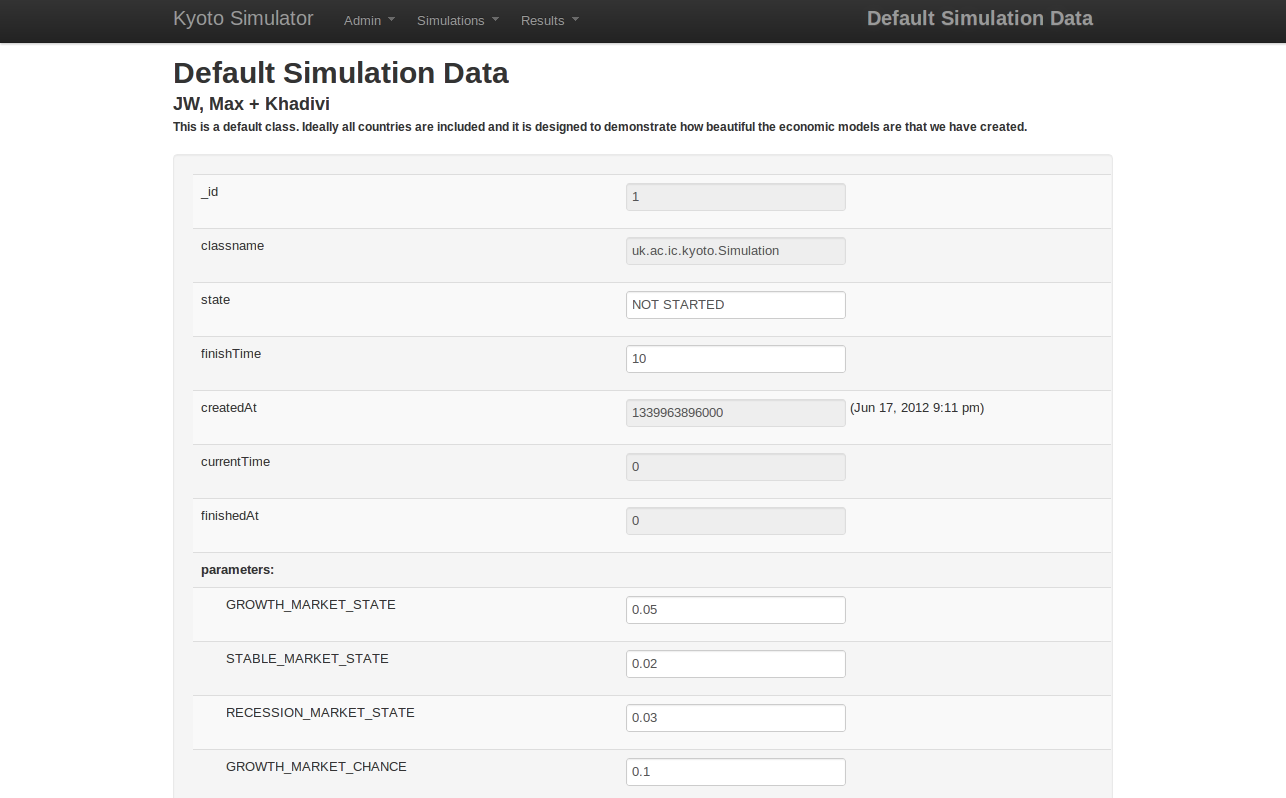
\includegraphics[width=0.9\textwidth]{img/ui3.png}
	\caption{}
\end{figure}
 
The simulation edit page is a low level editor for the simulation. Functionality is provided to rename the simulation, the simulation authors and all other simulation attributes which it makes sense to edit. It also provides a link to the country editor page (the simulation \textsc{id} is passed in the \textsc{url} to ensure editing takes place on the countries of the correct simulation).

\paragraph{Simulation Results} 

Data from the mongo database is extracted and processed into a compressed, standardised output form that is simpler to manipulate. Some of the data is collated to provide overall simulation statistics to be displayed on a results page.  Yearly data is used in conjunction with the Google Graph \textsc{api} to provide year by year moving analysis.  Trade data is extracted to form an overview of trading relations between countries.

\begin{figure}[h!]
	\centering
	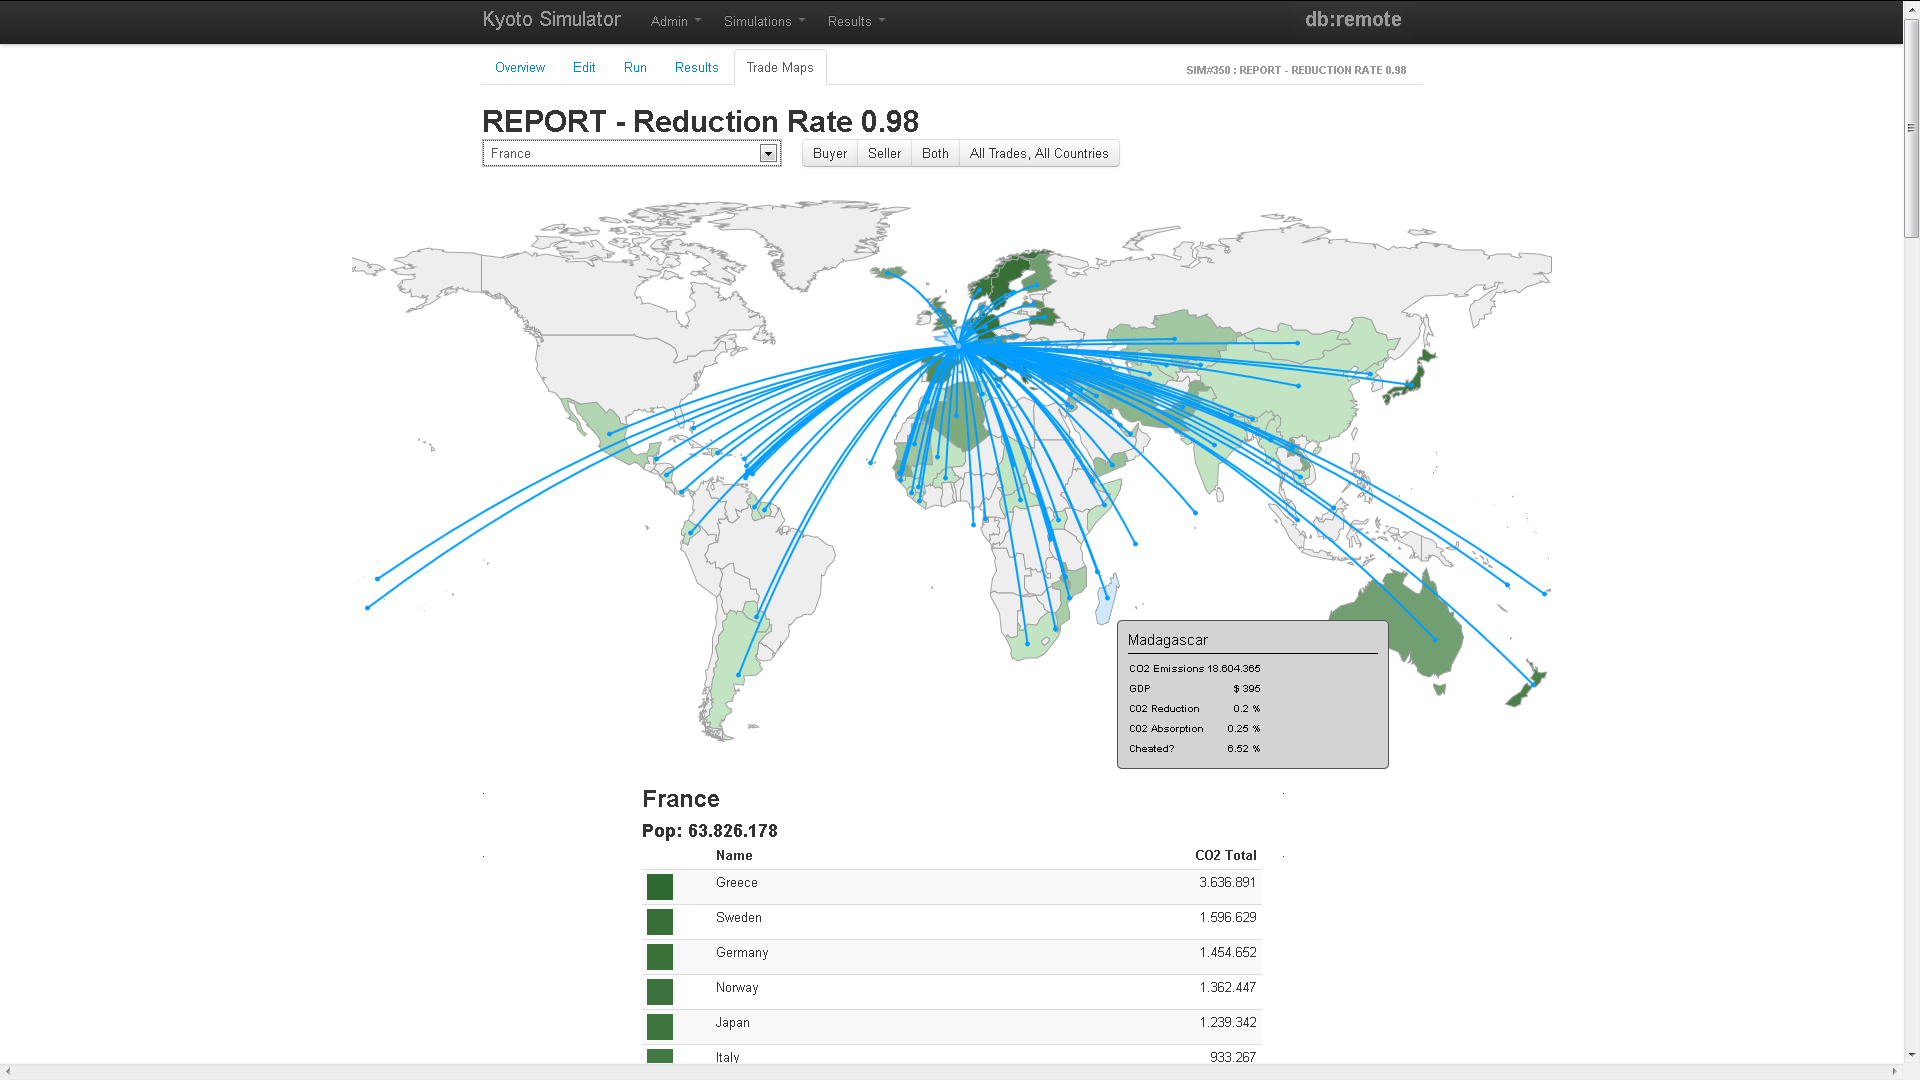
\includegraphics[width=0.9\textwidth]{img/franceGRAPH.png}
	\caption{KyotoUI illustating all trades which France has completed.}
\end{figure}
